\documentclass[1p]{elsarticle_modified}
%\bibliographystyle{elsarticle-num}

%\usepackage[colorlinks]{hyperref}
%\usepackage{abbrmath_seonhwa} %\Abb, \Ascr, \Acal ,\Abf, \Afrak
\usepackage{amsfonts}
\usepackage{amssymb}
\usepackage{amsmath}
\usepackage{amsthm}
\usepackage{scalefnt}
\usepackage{amsbsy}
\usepackage{kotex}
\usepackage{caption}
\usepackage{subfig}
\usepackage{color}
\usepackage{graphicx}
\usepackage{xcolor} %% white, black, red, green, blue, cyan, magenta, yellow
\usepackage{float}
\usepackage{setspace}
\usepackage{hyperref}

\usepackage{tikz}
\usetikzlibrary{arrows}

\usepackage{multirow}
\usepackage{array} % fixed length table
\usepackage{hhline}

%%%%%%%%%%%%%%%%%%%%%
\makeatletter
\renewcommand*\env@matrix[1][\arraystretch]{%
	\edef\arraystretch{#1}%
	\hskip -\arraycolsep
	\let\@ifnextchar\new@ifnextchar
	\array{*\c@MaxMatrixCols c}}
\makeatother %https://tex.stackexchange.com/questions/14071/how-can-i-increase-the-line-spacing-in-a-matrix
%%%%%%%%%%%%%%%

\usepackage[normalem]{ulem}

\newcommand{\msout}[1]{\ifmmode\text{\sout{\ensuremath{#1}}}\else\sout{#1}\fi}
%SOURCE: \msout is \stkout macro in https://tex.stackexchange.com/questions/20609/strikeout-in-math-mode

\newcommand{\cancel}[1]{
	\ifmmode
	{\color{red}\msout{#1}}
	\else
	{\color{red}\sout{#1}}
	\fi
}

\newcommand{\add}[1]{
	{\color{blue}\uwave{#1}}
}

\newcommand{\replace}[2]{
	\ifmmode
	{\color{red}\msout{#1}}{\color{blue}\uwave{#2}}
	\else
	{\color{red}\sout{#1}}{\color{blue}\uwave{#2}}
	\fi
}

\newcommand{\Sol}{\mathcal{S}} %segment
\newcommand{\D}{D} %diagram
\newcommand{\A}{\mathcal{A}} %arc


%%%%%%%%%%%%%%%%%%%%%%%%%%%%%5 test

\def\sl{\operatorname{\textup{SL}}(2,\Cbb)}
\def\psl{\operatorname{\textup{PSL}}(2,\Cbb)}
\def\quan{\mkern 1mu \triangleright \mkern 1mu}

\theoremstyle{definition}
\newtheorem{thm}{Theorem}[section]
\newtheorem{prop}[thm]{Proposition}
\newtheorem{lem}[thm]{Lemma}
\newtheorem{ques}[thm]{Question}
\newtheorem{cor}[thm]{Corollary}
\newtheorem{defn}[thm]{Definition}
\newtheorem{exam}[thm]{Example}
\newtheorem{rmk}[thm]{Remark}
\newtheorem{alg}[thm]{Algorithm}

\newcommand{\I}{\sqrt{-1}}
\begin{document}

%\begin{frontmatter}
%
%\title{Boundary parabolic representations of knots up to 8 crossings}
%
%%% Group authors per affiliation:
%\author{Yunhi Cho} 
%\address{Department of Mathematics, University of Seoul, Seoul, Korea}
%\ead{yhcho@uos.ac.kr}
%
%
%\author{Seonhwa Kim} %\fnref{s_kim}}
%\address{Center for Geometry and Physics, Institute for Basic Science, Pohang, 37673, Korea}
%\ead{ryeona17@ibs.re.kr}
%
%\author{Hyuk Kim}
%\address{Department of Mathematical Sciences, Seoul National University, Seoul 08826, Korea}
%\ead{hyukkim@snu.ac.kr}
%
%\author{Seokbeom Yoon}
%\address{Department of Mathematical Sciences, Seoul National University, Seoul, 08826,  Korea}
%\ead{sbyoon15@snu.ac.kr}
%
%\begin{abstract}
%We find all boundary parabolic representation of knots up to 8 crossings.
%
%\end{abstract}
%\begin{keyword}
%    \MSC[2010] 57M25 
%\end{keyword}
%
%\end{frontmatter}

%\linenumbers
%\tableofcontents
%
\newcommand\colored[1]{\textcolor{white}{\rule[-0.35ex]{0.8em}{1.4ex}}\kern-0.8em\color{red} #1}%
%\newcommand\colored[1]{\textcolor{white}{ #1}\kern-2.17ex	\textcolor{white}{ #1}\kern-1.81ex	\textcolor{white}{ #1}\kern-2.15ex\color{red}#1	}

{\Large $\underline{12n_{0256}~(K12n_{0256})}$}

\setlength{\tabcolsep}{10pt}
\renewcommand{\arraystretch}{1.6}
\vspace{1cm}\begin{tabular}{m{100pt}>{\centering\arraybackslash}m{274pt}}
\multirow{5}{120pt}{
	\centering
	\includegraphics[width=112pt]{../../../GIT/diagram.site/Diagrams/png/2345_12n_0256.png}\\
\ \ \ A knot diagram\footnotemark}&
\allowdisplaybreaks
\textbf{Linearized knot diagam} \\
\cline{2-2}
 &
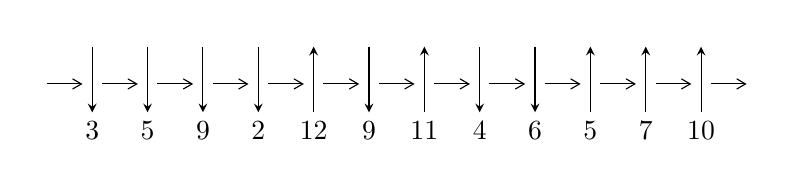
\begin{tikzpicture}[x=20pt, y=17pt]
	% nodes
	\node (C0) at (0, 0) {};
	\node (C1) at (1, 0) {};
	\node (C1U) at (1, +1) {};
	\node (C1D) at (1, -1) {3};

	\node (C2) at (2, 0) {};
	\node (C2U) at (2, +1) {};
	\node (C2D) at (2, -1) {5};

	\node (C3) at (3, 0) {};
	\node (C3U) at (3, +1) {};
	\node (C3D) at (3, -1) {9};

	\node (C4) at (4, 0) {};
	\node (C4U) at (4, +1) {};
	\node (C4D) at (4, -1) {2};

	\node (C5) at (5, 0) {};
	\node (C5U) at (5, +1) {};
	\node (C5D) at (5, -1) {12};

	\node (C6) at (6, 0) {};
	\node (C6U) at (6, +1) {};
	\node (C6D) at (6, -1) {9};

	\node (C7) at (7, 0) {};
	\node (C7U) at (7, +1) {};
	\node (C7D) at (7, -1) {11};

	\node (C8) at (8, 0) {};
	\node (C8U) at (8, +1) {};
	\node (C8D) at (8, -1) {4};

	\node (C9) at (9, 0) {};
	\node (C9U) at (9, +1) {};
	\node (C9D) at (9, -1) {6};

	\node (C10) at (10, 0) {};
	\node (C10U) at (10, +1) {};
	\node (C10D) at (10, -1) {5};

	\node (C11) at (11, 0) {};
	\node (C11U) at (11, +1) {};
	\node (C11D) at (11, -1) {7};

	\node (C12) at (12, 0) {};
	\node (C12U) at (12, +1) {};
	\node (C12D) at (12, -1) {10};
	\node (C13) at (13, 0) {};

	% arrows
	\draw[->,>={angle 60}]
	(C0) edge (C1) (C1) edge (C2) (C2) edge (C3) (C3) edge (C4) (C4) edge (C5) (C5) edge (C6) (C6) edge (C7) (C7) edge (C8) (C8) edge (C9) (C9) edge (C10) (C10) edge (C11) (C11) edge (C12) (C12) edge (C13) ;	\draw[->,>=stealth]
	(C1U) edge (C1D) (C2U) edge (C2D) (C3U) edge (C3D) (C4U) edge (C4D) (C5D) edge (C5U) (C6U) edge (C6D) (C7D) edge (C7U) (C8U) edge (C8D) (C9U) edge (C9D) (C10D) edge (C10U) (C11D) edge (C11U) (C12D) edge (C12U) ;
	\end{tikzpicture} \\
\hhline{~~} \\& 
\textbf{Solving Sequence} \\ \cline{2-2} 
 &
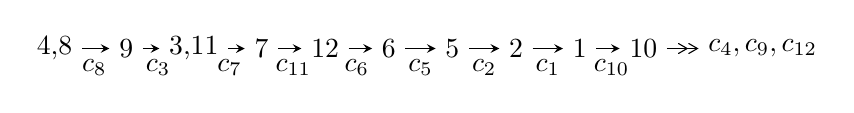
\begin{tikzpicture}[x=23pt, y=7pt]
	% node
	\node (A0) at (-1/8, 0) {4,8};
	\node (A1) at (1, 0) {9};
	\node (A2) at (33/16, 0) {3,11};
	\node (A3) at (25/8, 0) {7};
	\node (A4) at (33/8, 0) {12};
	\node (A5) at (41/8, 0) {6};
	\node (A6) at (49/8, 0) {5};
	\node (A7) at (57/8, 0) {2};
	\node (A8) at (65/8, 0) {1};
	\node (A9) at (73/8, 0) {10};
	\node (C1) at (1/2, -1) {$c_{8}$};
	\node (C2) at (3/2, -1) {$c_{3}$};
	\node (C3) at (21/8, -1) {$c_{7}$};
	\node (C4) at (29/8, -1) {$c_{11}$};
	\node (C5) at (37/8, -1) {$c_{6}$};
	\node (C6) at (45/8, -1) {$c_{5}$};
	\node (C7) at (53/8, -1) {$c_{2}$};
	\node (C8) at (61/8, -1) {$c_{1}$};
	\node (C9) at (69/8, -1) {$c_{10}$};
	\node (A10) at (11, 0) {$c_{4},c_{9},c_{12}$};

	% edge
	\draw[->,>=stealth]	
	(A0) edge (A1) (A1) edge (A2) (A2) edge (A3) (A3) edge (A4) (A4) edge (A5) (A5) edge (A6) (A6) edge (A7) (A7) edge (A8) (A8) edge (A9) ;
	\draw[->>,>={angle 60}]	
	(A9) edge (A10);
\end{tikzpicture} \\ 

\end{tabular} \\

\footnotetext{
The image of knot diagram is generated by the software ``\textbf{Draw programme}" developed by Andrew Bartholomew(\url{http://www.layer8.co.uk/maths/draw/index.htm\#Running-draw}), where we modified some parts for our purpose(\url{https://github.com/CATsTAILs/LinksPainter}).
}\phantom \\ \newline 
\centering \textbf{Ideals for irreducible components\footnotemark of $X_{\text{par}}$} 
 
\begin{align*}
I^u_{1}&=\langle 
-1.09302\times10^{148} u^{37}+5.18676\times10^{147} u^{36}+\cdots+1.58247\times10^{151} b-4.86012\times10^{152},\\
\phantom{I^u_{1}}&\phantom{= \langle  }2.92144\times10^{150} u^{37}-1.72552\times10^{150} u^{36}+\cdots+1.55082\times10^{153} a+1.44230\times10^{155},\\
\phantom{I^u_{1}}&\phantom{= \langle  }u^{38}- u^{37}+\cdots+86016 u-25088\rangle \\
I^u_{2}&=\langle 
-2796800274 u^{16}+1230170348 u^{15}+\cdots+5782655035 b+1488757467,\\
\phantom{I^u_{2}}&\phantom{= \langle  }8417711 u^{16}+1589468 u^{15}+\cdots+2844395 a-43377763,\;u^{17}+6 u^{15}+\cdots-3 u-1\rangle \\
\\
I^v_{1}&=\langle 
a,\;82026 v^8-2033115 v^7+\cdots+764761 b-1552510,\\
\phantom{I^v_{1}}&\phantom{= \langle  }7 v^9-3 v^8+2 v^7+14 v^6-23 v^5-33 v^4- v^3+8 v^2+v-1\rangle \\
\end{align*}
\raggedright * 3 irreducible components of $\dim_{\mathbb{C}}=0$, with total 64 representations.\\
\footnotetext{All coefficients of polynomials are rational numbers. But the coefficients are sometimes approximated in decimal forms when there is not enough margin.}
\newpage
\renewcommand{\arraystretch}{1}
\centering \section*{I. $I^u_{1}= \langle -1.09\times10^{148} u^{37}+5.19\times10^{147} u^{36}+\cdots+1.58\times10^{151} b-4.86\times10^{152},\;2.92\times10^{150} u^{37}-1.73\times10^{150} u^{36}+\cdots+1.55\times10^{153} a+1.44\times10^{155},\;u^{38}- u^{37}+\cdots+86016 u-25088 \rangle$}
\flushleft \textbf{(i) Arc colorings}\\
\begin{tabular}{m{7pt} m{180pt} m{7pt} m{180pt} }
\flushright $a_{4}=$&$\begin{pmatrix}0\\u\end{pmatrix}$ \\
\flushright $a_{8}=$&$\begin{pmatrix}1\\0\end{pmatrix}$ \\
\flushright $a_{9}=$&$\begin{pmatrix}1\\u^2\end{pmatrix}$ \\
\flushright $a_{3}=$&$\begin{pmatrix}u\\u^3+u\end{pmatrix}$ \\
\flushright $a_{11}=$&$\begin{pmatrix}-0.00188380 u^{37}+0.00111265 u^{36}+\cdots+197.770 u-93.0023\\0.000690707 u^{37}-0.000327764 u^{36}+\cdots-62.7881 u+30.7122\end{pmatrix}$ \\
\flushright $a_{7}=$&$\begin{pmatrix}0.000436226 u^{37}+0.0000991808 u^{36}+\cdots-6.16448 u+31.7162\\-0.000741300 u^{37}+0.000253145 u^{36}+\cdots+56.6644 u-36.9869\end{pmatrix}$ \\
\flushright $a_{12}=$&$\begin{pmatrix}-0.00175578 u^{37}+0.000884992 u^{36}+\cdots+151.445 u-59.3558\\0.00132438 u^{37}-0.000436480 u^{36}+\cdots-91.0821 u+52.7513\end{pmatrix}$ \\
\flushright $a_{6}=$&$\begin{pmatrix}-0.000858868 u^{37}+0.000550093 u^{36}+\cdots+85.6095 u-18.7030\\-0.00126665 u^{37}+0.000467679 u^{36}+\cdots+96.7862 u-58.1657\end{pmatrix}$ \\
\flushright $a_{5}=$&$\begin{pmatrix}-0.000317398 u^{37}+0.000185140 u^{36}+\cdots+29.3852 u-8.54883\\-0.0000363695 u^{37}+0.0000373746 u^{36}+\cdots+8.27143 u-5.50537\end{pmatrix}$ \\
\flushright $a_{2}=$&$\begin{pmatrix}0.000305502 u^{37}-0.000161572 u^{36}+\cdots-24.5272 u+6.36156\\0.0000100886 u^{37}+3.10588\times10^{-7} u^{36}+\cdots+0.142083 u+1.42366\end{pmatrix}$ \\
\flushright $a_{1}=$&$\begin{pmatrix}0.000281029 u^{37}-0.000147765 u^{36}+\cdots-21.1138 u+3.04347\\-0.0000370696 u^{37}+0.0000142949 u^{36}+\cdots+3.85910 u-2.16206\end{pmatrix}$ \\
\flushright $a_{10}=$&$\begin{pmatrix}-0.00191915 u^{37}+0.00125145 u^{36}+\cdots+217.235 u-96.5925\\0.000789868 u^{37}-0.000393658 u^{36}+\cdots-72.9083 u+33.0324\end{pmatrix}$\\&\end{tabular}
\flushleft \textbf{(ii) Obstruction class $= -1$}\\~\\
\flushleft \textbf{(iii) Cusp Shapes $= 0.00823228 u^{37}-0.00319378 u^{36}+\cdots-645.161 u+373.502$}\\~\\
\newpage\renewcommand{\arraystretch}{1}
\flushleft \textbf{(iv) u-Polynomials at the component}\newline \\
\begin{tabular}{m{50pt}|m{274pt}}
Crossings & \hspace{64pt}u-Polynomials at each crossing \\
\hline $$\begin{aligned}c_{1}\end{aligned}$$&$\begin{aligned}
&u^{38}+46 u^{36}+\cdots+6958 u+2401
\end{aligned}$\\
\hline $$\begin{aligned}c_{2},c_{4}\end{aligned}$$&$\begin{aligned}
&u^{38}-16 u^{37}+\cdots+378 u-49
\end{aligned}$\\
\hline $$\begin{aligned}c_{3},c_{8}\end{aligned}$$&$\begin{aligned}
&u^{38}- u^{37}+\cdots+86016 u-25088
\end{aligned}$\\
\hline $$\begin{aligned}c_{5}\end{aligned}$$&$\begin{aligned}
&u^{38}+4 u^{37}+\cdots-114 u-17
\end{aligned}$\\
\hline $$\begin{aligned}c_{6},c_{9}\end{aligned}$$&$\begin{aligned}
&u^{38}-3 u^{37}+\cdots-446 u+44
\end{aligned}$\\
\hline $$\begin{aligned}c_{7},c_{11}\end{aligned}$$&$\begin{aligned}
&u^{38}-2 u^{37}+\cdots-3904 u-5873
\end{aligned}$\\
\hline $$\begin{aligned}c_{10}\end{aligned}$$&$\begin{aligned}
&u^{38}+u^{37}+\cdots+40881797 u+3617129
\end{aligned}$\\
\hline $$\begin{aligned}c_{12}\end{aligned}$$&$\begin{aligned}
&u^{38}+u^{37}+\cdots+79046 u-14009
\end{aligned}$\\
\hline
\end{tabular}\\~\\
\newpage\renewcommand{\arraystretch}{1}
\flushleft \textbf{(v) Riley Polynomials at the component}\newline \\
\begin{tabular}{m{50pt}|m{274pt}}
Crossings & \hspace{64pt}Riley Polynomials at each crossing \\
\hline $$\begin{aligned}c_{1}\end{aligned}$$&$\begin{aligned}
&y^{38}+92 y^{37}+\cdots+262856678 y+5764801
\end{aligned}$\\
\hline $$\begin{aligned}c_{2},c_{4}\end{aligned}$$&$\begin{aligned}
&y^{38}+46 y^{36}+\cdots-6958 y+2401
\end{aligned}$\\
\hline $$\begin{aligned}c_{3},c_{8}\end{aligned}$$&$\begin{aligned}
&y^{38}+69 y^{37}+\cdots+3750756352 y+629407744
\end{aligned}$\\
\hline $$\begin{aligned}c_{5}\end{aligned}$$&$\begin{aligned}
&y^{38}-6 y^{37}+\cdots-8270 y+289
\end{aligned}$\\
\hline $$\begin{aligned}c_{6},c_{9}\end{aligned}$$&$\begin{aligned}
&y^{38}+35 y^{37}+\cdots-111884 y+1936
\end{aligned}$\\
\hline $$\begin{aligned}c_{7},c_{11}\end{aligned}$$&$\begin{aligned}
&y^{38}-12 y^{37}+\cdots-781291844 y+34492129
\end{aligned}$\\
\hline $$\begin{aligned}c_{10}\end{aligned}$$&$\begin{aligned}
&y^{38}-107 y^{37}+\cdots-346184004395873 y+13083622202641
\end{aligned}$\\
\hline $$\begin{aligned}c_{12}\end{aligned}$$&$\begin{aligned}
&y^{38}-69 y^{37}+\cdots-9544952050 y+196252081
\end{aligned}$\\
\hline
\end{tabular}\\~\\
\newpage\flushleft \textbf{(vi) Complex Volumes and Cusp Shapes}
$$\begin{array}{c|c|c}  
\text{Solutions to }I^u_{1}& \I (\text{vol} + \sqrt{-1}CS) & \text{Cusp shape}\\
 \hline 
\begin{aligned}
u &= -0.542649 + 0.614305 I \\
a &= -0.125480 + 0.480523 I \\
b &= \phantom{-}0.653832 + 0.819508 I\end{aligned}
 & \phantom{-}1.68943 + 7.69679 I & -0.16453 - 13.04445 I \\ \hline\begin{aligned}
u &= -0.542649 - 0.614305 I \\
a &= -0.125480 - 0.480523 I \\
b &= \phantom{-}0.653832 - 0.819508 I\end{aligned}
 & \phantom{-}1.68943 - 7.69679 I & -0.16453 + 13.04445 I \\ \hline\begin{aligned}
u &= \phantom{-}0.072090 + 0.744709 I \\
a &= \phantom{-}0.128090 - 1.010850 I \\
b &= \phantom{-}0.532310 - 0.601577 I\end{aligned}
 & \phantom{-}3.31755 + 0.54950 I & \phantom{-}6.15791 + 2.31967 I \\ \hline\begin{aligned}
u &= \phantom{-}0.072090 - 0.744709 I \\
a &= \phantom{-}0.128090 + 1.010850 I \\
b &= \phantom{-}0.532310 + 0.601577 I\end{aligned}
 & \phantom{-}3.31755 - 0.54950 I & \phantom{-}6.15791 - 2.31967 I \\ \hline\begin{aligned}
u &= -0.554003 + 0.499646 I \\
a &= \phantom{-}0.564998 + 0.241017 I \\
b &= \phantom{-}0.158389 - 0.923477 I\end{aligned}
 & -1.38624 + 1.33481 I & -2.97345 - 3.66862 I \\ \hline\begin{aligned}
u &= -0.554003 - 0.499646 I \\
a &= \phantom{-}0.564998 - 0.241017 I \\
b &= \phantom{-}0.158389 + 0.923477 I\end{aligned}
 & -1.38624 - 1.33481 I & -2.97345 + 3.66862 I \\ \hline\begin{aligned}
u &= \phantom{-}0.434969 + 0.601443 I \\
a &= \phantom{-}0.958601 - 0.178438 I \\
b &= -0.481321 - 0.092957 I\end{aligned}
 & \phantom{-}1.48961 + 0.57943 I & \phantom{-}5.02569 - 0.39325 I \\ \hline\begin{aligned}
u &= \phantom{-}0.434969 - 0.601443 I \\
a &= \phantom{-}0.958601 + 0.178438 I \\
b &= -0.481321 + 0.092957 I\end{aligned}
 & \phantom{-}1.48961 - 0.57943 I & \phantom{-}5.02569 + 0.39325 I \\ \hline\begin{aligned}
u &= \phantom{-}0.606671 + 0.412287 I \\
a &= \phantom{-}2.69689 + 1.44150 I \\
b &= -0.080725 + 1.288340 I\end{aligned}
 & -4.47346 + 0.84284 I & -11.66035 - 0.97344 I \\ \hline\begin{aligned}
u &= \phantom{-}0.606671 - 0.412287 I \\
a &= \phantom{-}2.69689 - 1.44150 I \\
b &= -0.080725 - 1.288340 I\end{aligned}
 & -4.47346 - 0.84284 I & -11.66035 + 0.97344 I\\
 \hline 
 \end{array}$$\newpage$$\begin{array}{c|c|c}  
\text{Solutions to }I^u_{1}& \I (\text{vol} + \sqrt{-1}CS) & \text{Cusp shape}\\
 \hline 
\begin{aligned}
u &= \phantom{-}0.185752 + 1.318190 I \\
a &= \phantom{-}0.527217 + 0.328502 I \\
b &= -0.165255 + 1.390640 I\end{aligned}
 & -2.12322 - 4.24125 I & -4.26882 + 3.51292 I \\ \hline\begin{aligned}
u &= \phantom{-}0.185752 - 1.318190 I \\
a &= \phantom{-}0.527217 - 0.328502 I \\
b &= -0.165255 - 1.390640 I\end{aligned}
 & -2.12322 + 4.24125 I & -4.26882 - 3.51292 I \\ \hline\begin{aligned}
u &= \phantom{-}0.626028 + 0.000453 I \\
a &= -0.113573 + 1.317400 I \\
b &= -0.686643 - 0.521082 I\end{aligned}
 & \phantom{-}0.61462 + 3.26287 I & -1.84851 - 7.14359 I \\ \hline\begin{aligned}
u &= \phantom{-}0.626028 - 0.000453 I \\
a &= -0.113573 - 1.317400 I \\
b &= -0.686643 + 0.521082 I\end{aligned}
 & \phantom{-}0.61462 - 3.26287 I & -1.84851 + 7.14359 I \\ \hline\begin{aligned}
u &= \phantom{-}0.220678 + 0.522522 I \\
a &= -7.64643 + 0.56839 I \\
b &= \phantom{-}0.541758 - 0.847309 I\end{aligned}
 & -0.41969 - 2.46857 I & \phantom{-}5.02234 + 6.21524 I \\ \hline\begin{aligned}
u &= \phantom{-}0.220678 - 0.522522 I \\
a &= -7.64643 - 0.56839 I \\
b &= \phantom{-}0.541758 + 0.847309 I\end{aligned}
 & -0.41969 + 2.46857 I & \phantom{-}5.02234 - 6.21524 I \\ \hline\begin{aligned}
u &= \phantom{-}0.134435 + 0.540176 I \\
a &= \phantom{-}0.616458 + 0.177082 I \\
b &= -0.685607 - 0.966646 I\end{aligned}
 & \phantom{-}0.34862 + 2.64648 I & \phantom{-}0.38453 - 4.62015 I \\ \hline\begin{aligned}
u &= \phantom{-}0.134435 - 0.540176 I \\
a &= \phantom{-}0.616458 - 0.177082 I \\
b &= -0.685607 + 0.966646 I\end{aligned}
 & \phantom{-}0.34862 - 2.64648 I & \phantom{-}0.38453 + 4.62015 I \\ \hline\begin{aligned}
u &= -0.487313\phantom{ +0.000000I} \\
a &= \phantom{-}1.16119\phantom{ +0.000000I} \\
b &= \phantom{-}0.259706\phantom{ +0.000000I}\end{aligned}
 & -1.21395\phantom{ +0.000000I} & -9.56810\phantom{ +0.000000I} \\ \hline\begin{aligned}
u &= -1.68632 + 0.08026 I \\
a &= \phantom{-}0.347568 - 0.381381 I \\
b &= -1.09335 - 0.89962 I\end{aligned}
 & \phantom{-}1.94242 + 0.25898 I & \phantom{-0.000000 } 0\\
 \hline 
 \end{array}$$\newpage$$\begin{array}{c|c|c}  
\text{Solutions to }I^u_{1}& \I (\text{vol} + \sqrt{-1}CS) & \text{Cusp shape}\\
 \hline 
\begin{aligned}
u &= -1.68632 - 0.08026 I \\
a &= \phantom{-}0.347568 + 0.381381 I \\
b &= -1.09335 + 0.89962 I\end{aligned}
 & \phantom{-}1.94242 - 0.25898 I & \phantom{-0.000000 } 0 \\ \hline\begin{aligned}
u &= \phantom{-}1.86202\phantom{ +0.000000I} \\
a &= \phantom{-}0.274789\phantom{ +0.000000I} \\
b &= -0.588779\phantom{ +0.000000I}\end{aligned}
 & -6.81012\phantom{ +0.000000I} & \phantom{-0.000000 } 0 \\ \hline\begin{aligned}
u &= -0.78573 + 1.74324 I \\
a &= -0.675257 + 0.449148 I \\
b &= \phantom{-}1.84271 + 0.04920 I\end{aligned}
 & \phantom{-}6.33444 - 4.25779 I & \phantom{-0.000000 } 0 \\ \hline\begin{aligned}
u &= -0.78573 - 1.74324 I \\
a &= -0.675257 - 0.449148 I \\
b &= \phantom{-}1.84271 - 0.04920 I\end{aligned}
 & \phantom{-}6.33444 + 4.25779 I & \phantom{-0.000000 } 0 \\ \hline\begin{aligned}
u &= \phantom{-}0.36940 + 1.96319 I \\
a &= -1.064530 - 0.184890 I \\
b &= \phantom{-}1.214130 - 0.199590 I\end{aligned}
 & \phantom{-}10.56750 - 4.02468 I & \phantom{-0.000000 } 0 \\ \hline\begin{aligned}
u &= \phantom{-}0.36940 - 1.96319 I \\
a &= -1.064530 + 0.184890 I \\
b &= \phantom{-}1.214130 + 0.199590 I\end{aligned}
 & \phantom{-}10.56750 + 4.02468 I & \phantom{-0.000000 } 0 \\ \hline\begin{aligned}
u &= \phantom{-}1.13922 + 2.02195 I \\
a &= \phantom{-}0.845877 + 0.411862 I \\
b &= -1.26404 + 1.60251 I\end{aligned}
 & \phantom{-}17.0081 - 15.1515 I & \phantom{-0.000000 } 0 \\ \hline\begin{aligned}
u &= \phantom{-}1.13922 - 2.02195 I \\
a &= \phantom{-}0.845877 - 0.411862 I \\
b &= -1.26404 - 1.60251 I\end{aligned}
 & \phantom{-}17.0081 + 15.1515 I & \phantom{-0.000000 } 0 \\ \hline\begin{aligned}
u &= -1.07898 + 2.08221 I \\
a &= \phantom{-}0.758885 - 0.409729 I \\
b &= -1.06379 - 1.81417 I\end{aligned}
 & \phantom{-}16.6139 + 6.3485 I & \phantom{-0.000000 } 0 \\ \hline\begin{aligned}
u &= -1.07898 - 2.08221 I \\
a &= \phantom{-}0.758885 + 0.409729 I \\
b &= -1.06379 + 1.81417 I\end{aligned}
 & \phantom{-}16.6139 - 6.3485 I & \phantom{-0.000000 } 0\\
 \hline 
 \end{array}$$\newpage$$\begin{array}{c|c|c}  
\text{Solutions to }I^u_{1}& \I (\text{vol} + \sqrt{-1}CS) & \text{Cusp shape}\\
 \hline 
\begin{aligned}
u &= \phantom{-}1.95530 + 1.96183 I \\
a &= -0.358887 - 0.264473 I \\
b &= \phantom{-}1.99385 + 0.02082 I\end{aligned}
 & \phantom{-}8.32107 - 2.64989 I & \phantom{-0.000000 } 0 \\ \hline\begin{aligned}
u &= \phantom{-}1.95530 - 1.96183 I \\
a &= -0.358887 + 0.264473 I \\
b &= \phantom{-}1.99385 - 0.02082 I\end{aligned}
 & \phantom{-}8.32107 + 2.64989 I & \phantom{-0.000000 } 0 \\ \hline\begin{aligned}
u &= -0.18789 + 2.88116 I \\
a &= \phantom{-}0.553430 - 0.032065 I \\
b &= -1.87447 + 1.62365 I\end{aligned}
 & \phantom{-}18.1843 + 3.4592 I & \phantom{-0.000000 } 0 \\ \hline\begin{aligned}
u &= -0.18789 - 2.88116 I \\
a &= \phantom{-}0.553430 + 0.032065 I \\
b &= -1.87447 - 1.62365 I\end{aligned}
 & \phantom{-}18.1843 - 3.4592 I & \phantom{-0.000000 } 0 \\ \hline\begin{aligned}
u &= -0.89301 + 2.76858 I \\
a &= -0.653362 + 0.138354 I \\
b &= \phantom{-}1.57197 + 0.58418 I\end{aligned}
 & \phantom{-}12.09730 + 5.36685 I & \phantom{-0.000000 } 0 \\ \hline\begin{aligned}
u &= -0.89301 - 2.76858 I \\
a &= -0.653362 - 0.138354 I \\
b &= \phantom{-}1.57197 - 0.58418 I\end{aligned}
 & \phantom{-}12.09730 - 5.36685 I & \phantom{-0.000000 } 0 \\ \hline\begin{aligned}
u &= -0.20333 + 3.10034 I \\
a &= \phantom{-}0.594985 - 0.039653 I \\
b &= -1.94922 - 1.37711 I\end{aligned}
 & \phantom{-}19.1617 + 5.3151 I & \phantom{-0.000000 } 0 \\ \hline\begin{aligned}
u &= -0.20333 - 3.10034 I \\
a &= \phantom{-}0.594985 + 0.039653 I \\
b &= -1.94922 + 1.37711 I\end{aligned}
 & \phantom{-}19.1617 - 5.3151 I & \phantom{-0.000000 } 0\\
 \hline 
 \end{array}$$\newpage\newpage\renewcommand{\arraystretch}{1}
\centering \section*{II. $I^u_{2}= \langle -2.80\times10^{9} u^{16}+1.23\times10^{9} u^{15}+\cdots+5.78\times10^{9} b+1.49\times10^{9},\;8.42\times10^{6} u^{16}+1.59\times10^{6} u^{15}+\cdots+2.84\times10^{6} a-4.34\times10^{7},\;u^{17}+6 u^{15}+\cdots-3 u-1 \rangle$}
\flushleft \textbf{(i) Arc colorings}\\
\begin{tabular}{m{7pt} m{180pt} m{7pt} m{180pt} }
\flushright $a_{4}=$&$\begin{pmatrix}0\\u\end{pmatrix}$ \\
\flushright $a_{8}=$&$\begin{pmatrix}1\\0\end{pmatrix}$ \\
\flushright $a_{9}=$&$\begin{pmatrix}1\\u^2\end{pmatrix}$ \\
\flushright $a_{3}=$&$\begin{pmatrix}u\\u^3+u\end{pmatrix}$ \\
\flushright $a_{11}=$&$\begin{pmatrix}-2.95940 u^{16}-0.558807 u^{15}+\cdots+7.83137 u+15.2503\\0.483653 u^{16}-0.212735 u^{15}+\cdots-1.67509 u-0.257452\end{pmatrix}$ \\
\flushright $a_{7}=$&$\begin{pmatrix}2.84567 u^{16}-2.41889 u^{15}+\cdots-21.8102 u+1.32723\\0.0829079 u^{16}-0.0995122 u^{15}+\cdots-1.83555 u-0.881897\end{pmatrix}$ \\
\flushright $a_{12}=$&$\begin{pmatrix}1.42944 u^{16}-2.13476 u^{15}+\cdots-12.9726 u+6.25927\\0.355787 u^{16}-0.159534 u^{15}+\cdots-2.01409 u-0.833403\end{pmatrix}$ \\
\flushright $a_{6}=$&$\begin{pmatrix}2.12965 u^{16}-2.32997 u^{15}+\cdots-19.2348 u+2.86422\\0.223987 u^{16}-0.211458 u^{15}+\cdots-2.28481 u-0.792978\end{pmatrix}$ \\
\flushright $a_{5}=$&$\begin{pmatrix}-1.08969 u^{16}+0.114263 u^{15}+\cdots+3.70066 u+2.95645\\0.141079 u^{16}-0.111945 u^{15}+\cdots-0.449264 u+0.0889186\end{pmatrix}$ \\
\flushright $a_{2}=$&$\begin{pmatrix}1.18986 u^{16}-0.118103 u^{15}+\cdots-3.40302 u-2.98180\\0.0172629 u^{16}+0.0956716 u^{15}+\cdots+1.13318 u-0.143448\end{pmatrix}$ \\
\flushright $a_{1}=$&$\begin{pmatrix}1.23077 u^{16}-0.226208 u^{15}+\cdots-4.14992 u-2.86754\\0.0648607 u^{16}+0.00369480 u^{15}+\cdots+0.102878 u-0.137290\end{pmatrix}$ \\
\flushright $a_{10}=$&$\begin{pmatrix}-4.27308 u^{16}-0.233087 u^{15}+\cdots+13.8168 u+17.9997\\0.377489 u^{16}-0.184057 u^{15}+\cdots-1.56233 u-0.0206505\end{pmatrix}$\\&\end{tabular}
\flushleft \textbf{(ii) Obstruction class $= 1$}\\~\\
\flushleft \textbf{(iii) Cusp Shapes $= \frac{45091796106}{5782655035} u^{16}-\frac{12435236787}{5782655035} u^{15}+\cdots-\frac{43331514147}{1156531007} u-\frac{96632179643}{5782655035}$}\\~\\
\newpage\renewcommand{\arraystretch}{1}
\flushleft \textbf{(iv) u-Polynomials at the component}\newline \\
\begin{tabular}{m{50pt}|m{274pt}}
Crossings & \hspace{64pt}u-Polynomials at each crossing \\
\hline $$\begin{aligned}c_{1}\end{aligned}$$&$\begin{aligned}
&u^{17}-8 u^{16}+\cdots+3 u-1
\end{aligned}$\\
\hline $$\begin{aligned}c_{2}\end{aligned}$$&$\begin{aligned}
&u^{17}+6 u^{16}+\cdots+u+1
\end{aligned}$\\
\hline $$\begin{aligned}c_{3}\end{aligned}$$&$\begin{aligned}
&u^{17}+6 u^{15}+\cdots-3 u+1
\end{aligned}$\\
\hline $$\begin{aligned}c_{4}\end{aligned}$$&$\begin{aligned}
&u^{17}-6 u^{16}+\cdots+u-1
\end{aligned}$\\
\hline $$\begin{aligned}c_{5}\end{aligned}$$&$\begin{aligned}
&u^{17}-6 u^{16}+\cdots+3 u-1
\end{aligned}$\\
\hline $$\begin{aligned}c_{6}\end{aligned}$$&$\begin{aligned}
&u^{17}-3 u^{16}+\cdots-6 u^2-1
\end{aligned}$\\
\hline $$\begin{aligned}c_{7}\end{aligned}$$&$\begin{aligned}
&u^{17}+6 u^{15}+\cdots+3 u+1
\end{aligned}$\\
\hline $$\begin{aligned}c_{8}\end{aligned}$$&$\begin{aligned}
&u^{17}+6 u^{15}+\cdots-3 u-1
\end{aligned}$\\
\hline $$\begin{aligned}c_{9}\end{aligned}$$&$\begin{aligned}
&u^{17}+3 u^{16}+\cdots+6 u^2+1
\end{aligned}$\\
\hline $$\begin{aligned}c_{10}\end{aligned}$$&$\begin{aligned}
&u^{17}+3 u^{16}+\cdots+6 u+1
\end{aligned}$\\
\hline $$\begin{aligned}c_{11}\end{aligned}$$&$\begin{aligned}
&u^{17}+6 u^{15}+\cdots+3 u-1
\end{aligned}$\\
\hline $$\begin{aligned}c_{12}\end{aligned}$$&$\begin{aligned}
&u^{17}-5 u^{16}+\cdots+5 u-1
\end{aligned}$\\
\hline
\end{tabular}\\~\\
\newpage\renewcommand{\arraystretch}{1}
\flushleft \textbf{(v) Riley Polynomials at the component}\newline \\
\begin{tabular}{m{50pt}|m{274pt}}
Crossings & \hspace{64pt}Riley Polynomials at each crossing \\
\hline $$\begin{aligned}c_{1}\end{aligned}$$&$\begin{aligned}
&y^{17}+8 y^{16}+\cdots-25 y-1
\end{aligned}$\\
\hline $$\begin{aligned}c_{2},c_{4}\end{aligned}$$&$\begin{aligned}
&y^{17}-8 y^{16}+\cdots+3 y-1
\end{aligned}$\\
\hline $$\begin{aligned}c_{3},c_{8}\end{aligned}$$&$\begin{aligned}
&y^{17}+12 y^{16}+\cdots+3 y-1
\end{aligned}$\\
\hline $$\begin{aligned}c_{5}\end{aligned}$$&$\begin{aligned}
&y^{17}+2 y^{16}+\cdots+19 y-1
\end{aligned}$\\
\hline $$\begin{aligned}c_{6},c_{9}\end{aligned}$$&$\begin{aligned}
&y^{17}+3 y^{16}+\cdots-12 y-1
\end{aligned}$\\
\hline $$\begin{aligned}c_{7},c_{11}\end{aligned}$$&$\begin{aligned}
&y^{17}+12 y^{16}+\cdots-3 y-1
\end{aligned}$\\
\hline $$\begin{aligned}c_{10}\end{aligned}$$&$\begin{aligned}
&y^{17}-19 y^{16}+\cdots-2 y-1
\end{aligned}$\\
\hline $$\begin{aligned}c_{12}\end{aligned}$$&$\begin{aligned}
&y^{17}-17 y^{16}+\cdots+7 y-1
\end{aligned}$\\
\hline
\end{tabular}\\~\\
\newpage\flushleft \textbf{(vi) Complex Volumes and Cusp Shapes}
$$\begin{array}{c|c|c}  
\text{Solutions to }I^u_{2}& \I (\text{vol} + \sqrt{-1}CS) & \text{Cusp shape}\\
 \hline 
\begin{aligned}
u &= \phantom{-}0.123817 + 0.916477 I \\
a &= -0.399407 + 0.909736 I \\
b &= -0.302924 + 0.816439 I\end{aligned}
 & \phantom{-}2.61790 - 2.40485 I & \phantom{-}3.33881 + 2.22795 I \\ \hline\begin{aligned}
u &= \phantom{-}0.123817 - 0.916477 I \\
a &= -0.399407 - 0.909736 I \\
b &= -0.302924 - 0.816439 I\end{aligned}
 & \phantom{-}2.61790 + 2.40485 I & \phantom{-}3.33881 - 2.22795 I \\ \hline\begin{aligned}
u &= -0.519605 + 0.973810 I \\
a &= -0.251920 - 0.419212 I \\
b &= -0.199212 - 0.760976 I\end{aligned}
 & \phantom{-}1.04490 + 6.61108 I & -1.52634 - 5.44334 I \\ \hline\begin{aligned}
u &= -0.519605 - 0.973810 I \\
a &= -0.251920 + 0.419212 I \\
b &= -0.199212 + 0.760976 I\end{aligned}
 & \phantom{-}1.04490 - 6.61108 I & -1.52634 + 5.44334 I \\ \hline\begin{aligned}
u &= -0.718697 + 0.273065 I \\
a &= \phantom{-}1.408880 - 0.113300 I \\
b &= -0.503625 + 0.659985 I\end{aligned}
 & \phantom{-}1.14952 - 2.21103 I & \phantom{-}2.23770 + 3.38646 I \\ \hline\begin{aligned}
u &= -0.718697 - 0.273065 I \\
a &= \phantom{-}1.408880 + 0.113300 I \\
b &= -0.503625 - 0.659985 I\end{aligned}
 & \phantom{-}1.14952 + 2.21103 I & \phantom{-}2.23770 - 3.38646 I \\ \hline\begin{aligned}
u &= \phantom{-}0.535223 + 1.162140 I \\
a &= -0.615278 - 0.480409 I \\
b &= -0.154895 - 1.305200 I\end{aligned}
 & -1.12324 - 5.07181 I & -0.31929 + 6.91281 I \\ \hline\begin{aligned}
u &= \phantom{-}0.535223 - 1.162140 I \\
a &= -0.615278 + 0.480409 I \\
b &= -0.154895 + 1.305200 I\end{aligned}
 & -1.12324 + 5.07181 I & -0.31929 - 6.91281 I \\ \hline\begin{aligned}
u &= -0.259361 + 1.266310 I \\
a &= -0.251583 + 0.034431 I \\
b &= -0.27641 + 1.42034 I\end{aligned}
 & \phantom{-}0.516364 - 0.300871 I & \phantom{-}0.207427 + 0.470649 I \\ \hline\begin{aligned}
u &= -0.259361 - 1.266310 I \\
a &= -0.251583 - 0.034431 I \\
b &= -0.27641 - 1.42034 I\end{aligned}
 & \phantom{-}0.516364 + 0.300871 I & \phantom{-}0.207427 - 0.470649 I\\
 \hline 
 \end{array}$$\newpage$$\begin{array}{c|c|c}  
\text{Solutions to }I^u_{2}& \I (\text{vol} + \sqrt{-1}CS) & \text{Cusp shape}\\
 \hline 
\begin{aligned}
u &= \phantom{-}0.642620 + 0.176331 I \\
a &= -0.79573 - 4.21005 I \\
b &= \phantom{-}0.06025 - 1.48960 I\end{aligned}
 & -3.99885 + 0.50220 I & -2.39894 + 6.28246 I \\ \hline\begin{aligned}
u &= \phantom{-}0.642620 - 0.176331 I \\
a &= -0.79573 + 4.21005 I \\
b &= \phantom{-}0.06025 + 1.48960 I\end{aligned}
 & -3.99885 - 0.50220 I & -2.39894 - 6.28246 I \\ \hline\begin{aligned}
u &= -0.314004 + 0.270023 I \\
a &= \phantom{-}12.21260 + 4.46195 I \\
b &= \phantom{-}0.368087 - 0.696391 I\end{aligned}
 & -0.26934 - 3.00568 I & -3.5088 - 14.7647 I \\ \hline\begin{aligned}
u &= -0.314004 - 0.270023 I \\
a &= \phantom{-}12.21260 - 4.46195 I \\
b &= \phantom{-}0.368087 + 0.696391 I\end{aligned}
 & -0.26934 + 3.00568 I & -3.5088 + 14.7647 I \\ \hline\begin{aligned}
u &= \phantom{-}1.73212\phantom{ +0.000000I} \\
a &= \phantom{-}0.299870\phantom{ +0.000000I} \\
b &= -0.404382\phantom{ +0.000000I}\end{aligned}
 & -6.94010\phantom{ +0.000000I} & -36.0810\phantom{ +0.000000I} \\ \hline\begin{aligned}
u &= -0.35606 + 2.09120 I \\
a &= -0.957501 + 0.103745 I \\
b &= \phantom{-}1.210930 + 0.258234 I\end{aligned}
 & \phantom{-}10.11250 + 4.21829 I & -4.98986 - 4.99941 I \\ \hline\begin{aligned}
u &= -0.35606 - 2.09120 I \\
a &= -0.957501 - 0.103745 I \\
b &= \phantom{-}1.210930 - 0.258234 I\end{aligned}
 & \phantom{-}10.11250 - 4.21829 I & -4.98986 + 4.99941 I\\
 \hline 
 \end{array}$$\newpage\newpage\renewcommand{\arraystretch}{1}
\centering \section*{III. $I^v_{1}= \langle a,\;8.20\times10^{4} v^{8}-2.03\times10^{6} v^{7}+\cdots+7.65\times10^{5} b-1.55\times10^{6},\;7 v^9-3 v^8+\cdots+v-1 \rangle$}
\flushleft \textbf{(i) Arc colorings}\\
\begin{tabular}{m{7pt} m{180pt} m{7pt} m{180pt} }
\flushright $a_{4}=$&$\begin{pmatrix}v\\0\end{pmatrix}$ \\
\flushright $a_{8}=$&$\begin{pmatrix}1\\0\end{pmatrix}$ \\
\flushright $a_{9}=$&$\begin{pmatrix}1\\0\end{pmatrix}$ \\
\flushright $a_{3}=$&$\begin{pmatrix}v\\0\end{pmatrix}$ \\
\flushright $a_{11}=$&$\begin{pmatrix}0\\-0.107257 v^{8}+2.65850 v^{7}+\cdots-0.280187 v+2.03006\end{pmatrix}$ \\
\flushright $a_{7}=$&$\begin{pmatrix}1\\2.14626 v^{8}+0.185889 v^{7}+\cdots-0.429870 v+1.30771\end{pmatrix}$ \\
\flushright $a_{12}=$&$\begin{pmatrix}-0.107257 v^{8}+2.65850 v^{7}+\cdots-0.280187 v+2.03006\\-1.38456 v^{8}+4.21937 v^{7}+\cdots-2.55986 v+1.77273\end{pmatrix}$ \\
\flushright $a_{6}=$&$\begin{pmatrix}2.14626 v^{8}+0.185889 v^{7}+\cdots-0.429870 v+2.30771\\2.14626 v^{8}+0.185889 v^{7}+\cdots-0.429870 v+1.30771\end{pmatrix}$ \\
\flushright $a_{5}=$&$\begin{pmatrix}-1.01346 v^{8}-0.464403 v^{7}+\cdots+1.07485 v+0.182471\\7 v^8-3 v^7+2 v^6+14 v^5-23 v^4-33 v^3- v^2+8 v+1\end{pmatrix}$ \\
\flushright $a_{2}=$&$\begin{pmatrix}1.01346 v^{8}+0.464403 v^{7}+\cdots-0.0748548 v-0.182471\\-7 v^8+3 v^7-2 v^6-14 v^5+23 v^4+33 v^3+v^2-8 v-1\end{pmatrix}$ \\
\flushright $a_{1}=$&$\begin{pmatrix}1.01346 v^{8}+0.464403 v^{7}+\cdots-1.07485 v-0.182471\\-7 v^8+3 v^7-2 v^6-14 v^5+23 v^4+33 v^3+v^2-8 v-1\end{pmatrix}$ \\
\flushright $a_{10}=$&$\begin{pmatrix}-5.30121 v^{8}+5.22147 v^{7}+\cdots-3.83160 v+0.359036\\-7.44747 v^{8}+5.03558 v^{7}+\cdots-3.40173 v-1.94867\end{pmatrix}$\\&\end{tabular}
\flushleft \textbf{(ii) Obstruction class $= 1$}\\~\\
\flushleft \textbf{(iii) Cusp Shapes $= -\frac{6992041}{764761} v^8+\frac{5331628}{764761} v^7-\frac{6285069}{764761} v^6-\frac{9541876}{764761} v^5+\frac{21850087}{764761} v^4+\frac{25370276}{764761} v^3-\frac{321417}{764761} v^2+\frac{135859}{764761} v+\frac{1854463}{764761}$}\\~\\
\newpage\renewcommand{\arraystretch}{1}
\flushleft \textbf{(iv) u-Polynomials at the component}\newline \\
\begin{tabular}{m{50pt}|m{274pt}}
Crossings & \hspace{64pt}u-Polynomials at each crossing \\
\hline $$\begin{aligned}c_{1},c_{2}\end{aligned}$$&$\begin{aligned}
&(u-1)^9
\end{aligned}$\\
\hline $$\begin{aligned}c_{3},c_{8}\end{aligned}$$&$\begin{aligned}
&u^9
\end{aligned}$\\
\hline $$\begin{aligned}c_{4}\end{aligned}$$&$\begin{aligned}
&(u+1)^9
\end{aligned}$\\
\hline $$\begin{aligned}c_{5}\end{aligned}$$&$\begin{aligned}
&u^9+5 u^8+12 u^7+15 u^6+9 u^5- u^4-4 u^3-2 u^2+u+1
\end{aligned}$\\
\hline $$\begin{aligned}c_{6}\end{aligned}$$&$\begin{aligned}
&u^9-3 u^8+8 u^7-13 u^6+17 u^5-17 u^4+12 u^3-6 u^2+u+1
\end{aligned}$\\
\hline $$\begin{aligned}c_{7}\end{aligned}$$&$\begin{aligned}
&u^9- u^8+2 u^7- u^6+3 u^5- u^4+2 u^3+u+1
\end{aligned}$\\
\hline $$\begin{aligned}c_{9}\end{aligned}$$&$\begin{aligned}
&u^9+3 u^8+8 u^7+13 u^6+17 u^5+17 u^4+12 u^3+6 u^2+u-1
\end{aligned}$\\
\hline $$\begin{aligned}c_{10},c_{12}\end{aligned}$$&$\begin{aligned}
&u^9+u^8-2 u^7-3 u^6+u^5+3 u^4+2 u^3- u-1
\end{aligned}$\\
\hline $$\begin{aligned}c_{11}\end{aligned}$$&$\begin{aligned}
&u^9+u^8+2 u^7+u^6+3 u^5+u^4+2 u^3+u-1
\end{aligned}$\\
\hline
\end{tabular}\\~\\
\newpage\renewcommand{\arraystretch}{1}
\flushleft \textbf{(v) Riley Polynomials at the component}\newline \\
\begin{tabular}{m{50pt}|m{274pt}}
Crossings & \hspace{64pt}Riley Polynomials at each crossing \\
\hline $$\begin{aligned}c_{1},c_{2},c_{4}\end{aligned}$$&$\begin{aligned}
&(y-1)^9
\end{aligned}$\\
\hline $$\begin{aligned}c_{3},c_{8}\end{aligned}$$&$\begin{aligned}
&y^9
\end{aligned}$\\
\hline $$\begin{aligned}c_{5}\end{aligned}$$&$\begin{aligned}
&y^9- y^8+12 y^7-7 y^6+37 y^5+y^4-10 y^2+5 y-1
\end{aligned}$\\
\hline $$\begin{aligned}c_{6},c_{9}\end{aligned}$$&$\begin{aligned}
&y^9+7 y^8+20 y^7+25 y^6+5 y^5-15 y^4+22 y^2+13 y-1
\end{aligned}$\\
\hline $$\begin{aligned}c_{7},c_{11}\end{aligned}$$&$\begin{aligned}
&y^9+3 y^8+8 y^7+13 y^6+17 y^5+17 y^4+12 y^3+6 y^2+y-1
\end{aligned}$\\
\hline $$\begin{aligned}c_{10},c_{12}\end{aligned}$$&$\begin{aligned}
&y^9-5 y^8+12 y^7-15 y^6+9 y^5+y^4-4 y^3+2 y^2+y-1
\end{aligned}$\\
\hline
\end{tabular}\\~\\
\newpage\flushleft \textbf{(vi) Complex Volumes and Cusp Shapes}
$$\begin{array}{c|c|c}  
\text{Solutions to }I^v_{1}& \I (\text{vol} + \sqrt{-1}CS) & \text{Cusp shape}\\
 \hline 
\begin{aligned}
v &= -0.903964 + 0.094390 I \\
a &= \phantom{-0.000000 } 0 \\
b &= -0.140343 + 0.966856 I\end{aligned}
 & -3.42837 - 2.09337 I & -6.52230 + 4.24226 I \\ \hline\begin{aligned}
v &= -0.903964 - 0.094390 I \\
a &= \phantom{-0.000000 } 0 \\
b &= -0.140343 - 0.966856 I\end{aligned}
 & -3.42837 + 2.09337 I & -6.52230 - 4.24226 I \\ \hline\begin{aligned}
v &= \phantom{-}1.42091\phantom{ +0.000000I} \\
a &= \phantom{-0.000000 } 0 \\
b &= -0.512358\phantom{ +0.000000I}\end{aligned}
 & -0.446489\phantom{ +0.000000I} & \phantom{-}3.16660\phantom{ +0.000000I} \\ \hline\begin{aligned}
v &= -0.476406 + 0.294981 I \\
a &= \phantom{-0.000000 } 0 \\
b &= \phantom{-}0.796005 + 0.733148 I\end{aligned}
 & \phantom{-}2.72642 - 1.33617 I & \phantom{-}0.84367 + 3.27176 I \\ \hline\begin{aligned}
v &= -0.476406 - 0.294981 I \\
a &= \phantom{-0.000000 } 0 \\
b &= \phantom{-}0.796005 - 0.733148 I\end{aligned}
 & \phantom{-}2.72642 + 1.33617 I & \phantom{-}0.84367 - 3.27176 I \\ \hline\begin{aligned}
v &= \phantom{-}0.352455 + 0.113243 I \\
a &= \phantom{-0.000000 } 0 \\
b &= \phantom{-}0.728966 - 0.986295 I\end{aligned}
 & \phantom{-}1.95319 - 7.08493 I & \phantom{-}3.61934 + 1.74309 I \\ \hline\begin{aligned}
v &= \phantom{-}0.352455 - 0.113243 I \\
a &= \phantom{-0.000000 } 0 \\
b &= \phantom{-}0.728966 + 0.986295 I\end{aligned}
 & \phantom{-}1.95319 + 7.08493 I & \phantom{-}3.61934 - 1.74309 I \\ \hline\begin{aligned}
v &= \phantom{-}0.53175 + 1.59553 I \\
a &= \phantom{-0.000000 } 0 \\
b &= -0.628449 + 0.875112 I\end{aligned}
 & -1.02799 - 2.45442 I & -8.21790 + 4.39771 I \\ \hline\begin{aligned}
v &= \phantom{-}0.53175 - 1.59553 I \\
a &= \phantom{-0.000000 } 0 \\
b &= -0.628449 - 0.875112 I\end{aligned}
 & -1.02799 + 2.45442 I & -8.21790 - 4.39771 I\\
 \hline 
 \end{array}$$\newpage
\newpage\renewcommand{\arraystretch}{1}
\centering \section*{ IV. u-Polynomials}
\begin{tabular}{m{50pt}|m{274pt}}
Crossings & \hspace{64pt}u-Polynomials at each crossing \\
\hline $$\begin{aligned}c_{1}\end{aligned}$$&$\begin{aligned}
&((u-1)^9)(u^{17}-8 u^{16}+\cdots+3 u-1)(u^{38}+46 u^{36}+\cdots+6958 u+2401)
\end{aligned}$\\
\hline $$\begin{aligned}c_{2}\end{aligned}$$&$\begin{aligned}
&((u-1)^9)(u^{17}+6 u^{16}+\cdots+u+1)(u^{38}-16 u^{37}+\cdots+378 u-49)
\end{aligned}$\\
\hline $$\begin{aligned}c_{3}\end{aligned}$$&$\begin{aligned}
&u^9(u^{17}+6 u^{15}+\cdots-3 u+1)(u^{38}-u^{37}+\cdots+86016 u-25088)
\end{aligned}$\\
\hline $$\begin{aligned}c_{4}\end{aligned}$$&$\begin{aligned}
&((u+1)^9)(u^{17}-6 u^{16}+\cdots+u-1)(u^{38}-16 u^{37}+\cdots+378 u-49)
\end{aligned}$\\
\hline $$\begin{aligned}c_{5}\end{aligned}$$&$\begin{aligned}
&(u^9+5 u^8+12 u^7+15 u^6+9 u^5- u^4-4 u^3-2 u^2+u+1)\\
&\cdot(u^{17}-6 u^{16}+\cdots+3 u-1)(u^{38}+4 u^{37}+\cdots-114 u-17)
\end{aligned}$\\
\hline $$\begin{aligned}c_{6}\end{aligned}$$&$\begin{aligned}
&(u^9-3 u^8+8 u^7-13 u^6+17 u^5-17 u^4+12 u^3-6 u^2+u+1)\\
&\cdot(u^{17}-3 u^{16}+\cdots-6 u^2-1)(u^{38}-3 u^{37}+\cdots-446 u+44)
\end{aligned}$\\
\hline $$\begin{aligned}c_{7}\end{aligned}$$&$\begin{aligned}
&(u^9- u^8+\cdots+u+1)(u^{17}+6 u^{15}+\cdots+3 u+1)\\
&\cdot(u^{38}-2 u^{37}+\cdots-3904 u-5873)
\end{aligned}$\\
\hline $$\begin{aligned}c_{8}\end{aligned}$$&$\begin{aligned}
&u^9(u^{17}+6 u^{15}+\cdots-3 u-1)(u^{38}-u^{37}+\cdots+86016 u-25088)
\end{aligned}$\\
\hline $$\begin{aligned}c_{9}\end{aligned}$$&$\begin{aligned}
&(u^9+3 u^8+8 u^7+13 u^6+17 u^5+17 u^4+12 u^3+6 u^2+u-1)\\
&\cdot(u^{17}+3 u^{16}+\cdots+6 u^2+1)(u^{38}-3 u^{37}+\cdots-446 u+44)
\end{aligned}$\\
\hline $$\begin{aligned}c_{10}\end{aligned}$$&$\begin{aligned}
&(u^9+u^8+\cdots- u-1)(u^{17}+3 u^{16}+\cdots+6 u+1)\\
&\cdot(u^{38}+u^{37}+\cdots+40881797 u+3617129)
\end{aligned}$\\
\hline $$\begin{aligned}c_{11}\end{aligned}$$&$\begin{aligned}
&(u^9+u^8+\cdots+u-1)(u^{17}+6 u^{15}+\cdots+3 u-1)\\
&\cdot(u^{38}-2 u^{37}+\cdots-3904 u-5873)
\end{aligned}$\\
\hline $$\begin{aligned}c_{12}\end{aligned}$$&$\begin{aligned}
&(u^9+u^8+\cdots- u-1)(u^{17}-5 u^{16}+\cdots+5 u-1)\\
&\cdot(u^{38}+u^{37}+\cdots+79046 u-14009)
\end{aligned}$\\
\hline
\end{tabular}\newpage\renewcommand{\arraystretch}{1}
\centering \section*{ V. Riley Polynomials}
\begin{tabular}{m{50pt}|m{274pt}}
Crossings & \hspace{64pt}Riley Polynomials at each crossing \\
\hline $$\begin{aligned}c_{1}\end{aligned}$$&$\begin{aligned}
&((y-1)^9)(y^{17}+8 y^{16}+\cdots-25 y-1)\\
&\cdot(y^{38}+92 y^{37}+\cdots+262856678 y+5764801)
\end{aligned}$\\
\hline $$\begin{aligned}c_{2},c_{4}\end{aligned}$$&$\begin{aligned}
&((y-1)^9)(y^{17}-8 y^{16}+\cdots+3 y-1)(y^{38}+46 y^{36}+\cdots-6958 y+2401)
\end{aligned}$\\
\hline $$\begin{aligned}c_{3},c_{8}\end{aligned}$$&$\begin{aligned}
&y^9(y^{17}+12 y^{16}+\cdots+3 y-1)\\
&\cdot(y^{38}+69 y^{37}+\cdots+3750756352 y+629407744)
\end{aligned}$\\
\hline $$\begin{aligned}c_{5}\end{aligned}$$&$\begin{aligned}
&(y^9- y^8+12 y^7-7 y^6+37 y^5+y^4-10 y^2+5 y-1)\\
&\cdot(y^{17}+2 y^{16}+\cdots+19 y-1)(y^{38}-6 y^{37}+\cdots-8270 y+289)
\end{aligned}$\\
\hline $$\begin{aligned}c_{6},c_{9}\end{aligned}$$&$\begin{aligned}
&(y^9+7 y^8+20 y^7+25 y^6+5 y^5-15 y^4+22 y^2+13 y-1)\\
&\cdot(y^{17}+3 y^{16}+\cdots-12 y-1)(y^{38}+35 y^{37}+\cdots-111884 y+1936)
\end{aligned}$\\
\hline $$\begin{aligned}c_{7},c_{11}\end{aligned}$$&$\begin{aligned}
&(y^9+3 y^8+8 y^7+13 y^6+17 y^5+17 y^4+12 y^3+6 y^2+y-1)\\
&\cdot(y^{17}+12 y^{16}+\cdots-3 y-1)\\
&\cdot(y^{38}-12 y^{37}+\cdots-781291844 y+34492129)
\end{aligned}$\\
\hline $$\begin{aligned}c_{10}\end{aligned}$$&$\begin{aligned}
&(y^9-5 y^8+12 y^7-15 y^6+9 y^5+y^4-4 y^3+2 y^2+y-1)\\
&\cdot(y^{17}-19 y^{16}+\cdots-2 y-1)\\
&\cdot(y^{38}-107 y^{37}+\cdots-346184004395873 y+13083622202641)
\end{aligned}$\\
\hline $$\begin{aligned}c_{12}\end{aligned}$$&$\begin{aligned}
&(y^9-5 y^8+12 y^7-15 y^6+9 y^5+y^4-4 y^3+2 y^2+y-1)\\
&\cdot(y^{17}-17 y^{16}+\cdots+7 y-1)\\
&\cdot(y^{38}-69 y^{37}+\cdots-9544952050 y+196252081)
\end{aligned}$\\
\hline
\end{tabular}
\vskip 2pc
\end{document}